\chapter{Implementace}
% TODO: napsat přehled, co bude v této kapitole

\section{Specifikace pravidel požadovaných zadáním práce}
Pro specifikaci Demeter law definujeme predikát, který nám umožní vybrat vhodné množiny vrcholů. Vybrané množiny potom ověřeíme pomocí predikátu, který učí, zda jsou tyto množiny v pořádku, či zda porušují LoD princip.

% TODO: přidat ukázková jenoduchá pravidla (a la PMD) pro demonstraci toho, že to program taky zvládne (např. limity na počty parametrů nebo členských proměnných ve třídě)

\begin{definition}
Mějme graf $G = \langle V, E, \rho, K, C, \mathit{Kind}, \mathit{Class}\rangle$ se zobrazeními definovanými dříve. Definujme selektor $F(G, v', k', c')$, $v' \in V$, $k' \in K$, $c' \in C$ jako množinu vrcholů grafu $G$, které jsou dostupné z vrcholu $v'$ pomocí orientované cesty, pro jejíž všechny vrcholy $v''$ s~výjimkou posledního platí $Kind(v) \ne k'$ a která obsahuje hranu $e$, pro niž platí $Class(e) = c' $.
\end{definition}

\subsection{Law of Demeter}
Pro provedení validace princip LoD využijeme graf podobný tomu na obrázku \ref{implementation-lod_graph}. Lze jej získat ze zdrojových kódů pogramu. Vazba $\langle\langle{}uses\rangle\rangle$ představuje všechna použití (přístup k~public a protected polím a volání metod) jiných tříd v rámci metody.

\begin{figure}[h!]
  \centering
  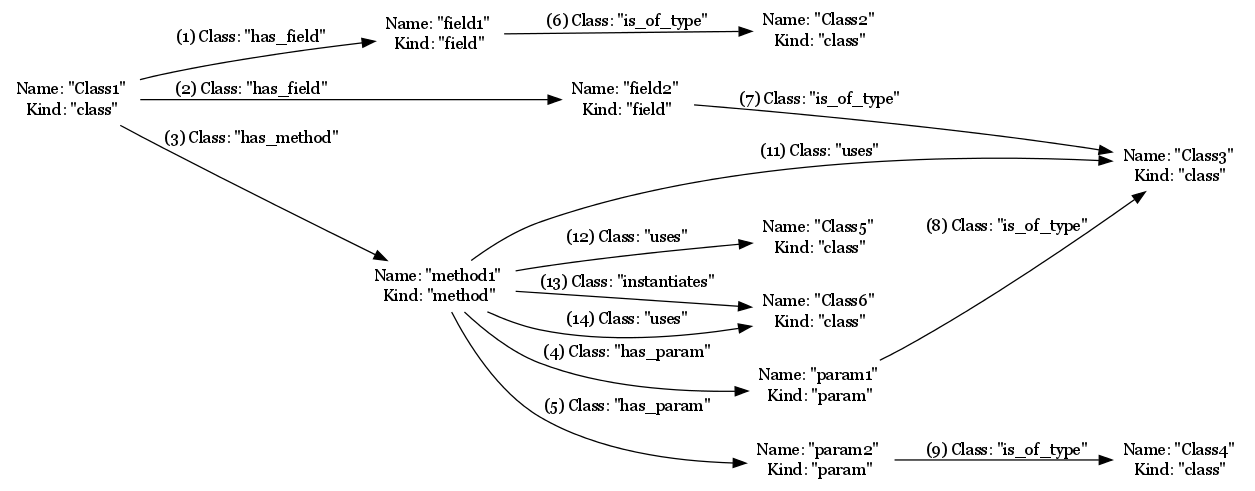
\includegraphics[width=1.0\textwidth]{./graphs/demeter_graph.png}
  \caption{Graf použitý pro validaci principu LoD.\label{implementation-lod_graph}}
\end{figure}

Pravidlo LoD potom specifikujeme nad grafem $G = \langle V, E, \rho, K, C, \mathit{Kind}, \mathit{Class}\rangle$ následovně:

\begin{align*}
\forall v \in V: Kind(v) = class\\
\end{align*}
\begin{align*}
[((&F(G, v, class, \langle\langle{}has\_field\rangle\rangle{}) \cup F(G, v, class, \langle\langle{}has\_param\rangle\rangle{}) \cup\\
&F(G, v, class, \langle\langle{}instantiates\rangle\rangle{})) \cap F(v, class, \langle\langle{}uses\rangle\rangle{}) \setminus \{v\}] = \emptyset
\end{align*}

Specifikované pravidlo vyjadřuje požadavek, aby množina vrcholů do níž se dostaneme pomocí hran, které představují povolené vstupy tříd do analyzované třídy (třídní proměnné, parametry, vytvářené objekty), byla totožná s množinou všech vrcholů, které představují všechny třídy používané (klasifikátor $\langle\langle{}uses\rangle\rangle$) v rámci některé z metod. Odečtení vrcholu $v$ z výsledné množiny je zde kvůli tomu, abychom nemuseli navíc zavádět zbytečnou hranu identifikující, že třída je známá sama sobě.

\subsection{Low coupling}
% TODO:
%% ## Typy závislostí mezi třídami

%% * třída A dědí ze třídy B
%% * třída A provádí instanciaci třídy B
%% * třída A používá existující intanci třídy B (pracuje s referencí na tuto třídu)

%% Na základě těchto závislostí lze sestavit orientovaný graf. Hrany budeme dále klasifikovat podle toho, o jakou závislost se jedná (dědičnost vs. vyvolání metody).

\subsection{High cohesion}
% TODO:

\section{Implementace jádra systému}
% TODO: describe technologies used to implement parser and analysis part
% TODO: moduly popsané v části \ref{design-architecture} implementujeme jako jednotlivé moduly platformy NetBeans.

\subsection{Implementace registrů poskytovatelů služeb}
\begin{itemize}
\item SPI
\item NetBeans lookup -- /META-INF/services
\end{itemize}

\subsection{Implementace základních operátorů}
Vyhodnocení univerzálního kvantifikátoru $\forall v \in V$ lze přepsat jako jednoduchý cyklus přes vrcholy vrácené zpřesňující operátorem, která vybírá nějakou podmnožinu z množiny vrcholů analyzovaného grafu. Získáme tak kód podobný listingu \ref{listing-forall}. V tomto kódu, který je fragmentem metody používáme symoblický název \verb+condition+ pro podmínku, kterou musí splňovat každý prvek \emph{v} iterované kolekce vrcholů \emph{vertices}.

\begin{lstlisting}[
    language=java,
    caption={Implementace univerzálního kvantifikátoru $\forall$.},
    label=listing-forall
  ]
for (Vertex v : vertices) {
    if (!condition(v, ...)) {
        return false;
    }
}
return true;
\end{lstlisting}

Analogicky budeme postupovat u existenčního kvantifikátoru $\exists$. Zde nám stačí nalézt alespoň jeden element, pro který vyhodnocovaná vlastnost platí. Listing \ref{listing-exists} představuje fragment metody. Pokud se podaří nalézt alespoň jeden prvek, který splňuje požadovanou podmínku, metoda vrátí hodnotu \emph{true}. Vzhledem k použití příkazu \emph{return} je zřejmé, že dochází k \uv{línemu} vyhodnocování -- vyhodnocení je ukončeno nalezením prvního vyhovujícího elementu (další se neprohledávají). Stejně jako u operátoru $\forall$ i zde název \verb+condition+ symbolizuje konkrétní podmínku, která má platit nad alespoň jedním prvkem množiny uzlů.

\begin{lstlisting}[
    language=java,
    caption={Implementace existenčního kvantifikátoru $\exists$.},
    label=listing-exists
  ]
for (Vertex v : vertices) {
    if (condition(v, ..)) {
        return true;
    }
}
return false;
\end{lstlisting}

Můžeme si všimnout, že se obě implementace liší pouze přehozením podmínek -- zatímco v prvním případě ($\forall$) musíme projít všechny prvky, abychom zjistili, zda všechny prvky splňují požadovanou vlastnost, ve druhém případě ($\exists$) budeme všechny prvky procházet pouze v krajním případě, kdy vlastnost neplatí pro žádný z prvků.

% TODO: přesunout do sekce týkající se generátorů grafu (možná dokonce do návrhu nebo analýzy)
% TODO: roztřídit
\begin{itemize}
\item Java 6 Compiler API (JSR 199) \cite{apidoc:java6api}
\item annotation processor (JSR 269)
\item Compiler Tree API
  \begin{itemize}
  \item \verb+com.sun.source.tree+
  \item \verb+com.sun.source.util+
  \end{itemize}
\item je nutné použít nestandardní API, které je součástí Sun Javy - balíčky \verb+com.sun.*+ (je potřeba přidat \$\{java\_home\}/../lib/tools.jar do classpath)
\end{itemize}

\section{Implementace modulů rozšíření}

\subsection{av-graphgen-demeter}
ukázkový poskytovatel generátoru grafu

\emph{DemeterGraphGeneratorProvider} implementuje \emph{GraphGeneratorIface}.

\subsection{av-operators-demeter}
ukázkový balíček operátorů pro ověřování principu LoD

Obsahuje sadu tříd implementující operátory potřebné pro definování pravidla pro validaci LoD. Tyto třídy implementují rozhraní \subsubsection{OperatorIface} (resp. jeho podtypy).

\subsection{av-analysis-lowcoup}
ukázková analýza low coupling

\subsection{av-analysis-highcoh}
ukázková analýza high cohesion

\section{Integrace do NetBeans IDE}

Při implementaci bylo hojně využíváno informací z \cite{netbeans_platform}.

% TODO: write about actions, about usage of the ArchVal API
Seznam integračních komponent je k dispozici v tabulce \ref{implementation-integration_components}.

\begin{table}
  \caption{Tabulka integračních komponent systému. \label{implementation-integration_components}}
  \begin{center}
    \begin{tabular}{ | l | l | p{8cm} | }
      \hline
      \textbf{Název} & \textbf{Typ} & \textbf{Zodpovědnost} \\
      \hline
      \hline
      Action & class & integrace s běhovou platformou, vstupní/aktivační bod \\ \hline
      %% TODO: 'třída implementující rozhraní...'
      GraphGeneratorRegister & class & třída poskytující přístup k informacím o existujících poskytovatelích generátorů grafu \\ \hline
      OperatorRegister & class & třída poskytující přístup k informacím o existujících poskytovatelích operátorů \\ \hline
      AnalysesRegister & class & třída poskytující přístup k informacím o existujících poskytovatelích komponent analýzy \\ \hline
      OutputGeneratorRegister & class & třída poskytující přístup k informacím o existujících poskytovatelích generátorů výstupních reportů \\ \hline
    \end{tabular}
  \end{center}
\end{table}

\subsection{Action}
Integrace do běhové platformy. Reprezentuje uživatelskou akci. Bude implementováno na základě zvolené implementační platformy (akce v GUI).

\subsection{Podpora editace AVD souborů}
\begin{itemize}
\item experimentální mime typ \verb+text/x-avd+
\item zvýrazňování syntaxe
\end{itemize}

\subsection{Výstupní rozhraní}
Podpora pro různé formáty výstupu. Popsat vnitřní reprezentaci reportu, tak aby jej bylo možné převést na vhodnou vnější reprezentaci. Podpora pro dopsání různých výstupních formátu jako např.:
\begin{itemize}
\item HTML
\item prostý text
\item zobrazení pomocí swing komponent (vygenerování modelu pro JTree)
\item \ldots
\end{itemize}

\subsection{Konfigurace}
\begin{itemize}
\item konfigurovatelné položky
\item konfigurační dialog
\item způsob ukládání konfigurace (podporováno platformou NB)
\end{itemize}
